\section{Serial Data Transfer Exercises}

\subsection{UART Communication}

\begin{KR}{Analyzing UART Transmission}
\paragraph{Determine bit timing}
\begin{itemize}
    \item Calculate bit period (T) from baud rate: T = 1/baud\_rate
    \item Example: 19200 baud = 1/19200 s = 52.1 µs per bit
\end{itemize}

\paragraph{Identify frame structure}
\begin{itemize}
    \item Start bit: Always '0'
    \item Data bits: LSB first, typically 7 or 8 bits
    \item Parity bit: Optional, can be even, odd, mark ('1'), or space ('0')
    \item Stop bit(s): Always '1', can be 1, 1.5, or 2 bits
    \item Idle state: Line remains high ('1')
\end{itemize}

\paragraph{Calculate total frame time}
\begin{itemize}
    \item Add up all bits: Start bit + Data bits + Parity bit + Stop bits
    \item Multiply by bit period (T)
    \item Example: 8N1 (8 data bits, no parity, 1 stop bit) = 10 bits total
\end{itemize}

\paragraph{Calculate maximum throughput}
\begin{itemize}
    \item Divide baud rate by total number of bits per frame
    \item Example: 9600 baud, 8N1 format = 9600/10 = 960 bytes/second
\end{itemize}

\paragraph{Evaluate clock tolerance}
\begin{itemize}
    \item Maximum tolerable deviation is typically ±(0.5/n) where n is the number of bits from start bit to the last data bit
    \item Example: For 8 data bits, max deviation = ±(0.5/8.5) $\approx$ ±5.9\%
\end{itemize}
\end{KR}

\begin{example2}{UART Transmission Analysis}\\
For a UART transmission with 19,200 bits/s, 7 data bits, and one stop bit (no parity), draw the timing diagram for transmitting the ASCII characters "AC".

ASCII values:
\begin{itemize}
    \item 'A' = 0x41 = 100 0001b
    \item 'C' = 0x43 = 100 0011b
\end{itemize}

\tcblower
\paragraph{Solution:}
First, calculate the bit period:
\begin{itemize}
    \item T = 1/19200 s = 52.1 µs
\end{itemize}

For each character, the frame consists of:
\begin{itemize}
    \item 1 start bit (S) - always '0'
    \item 7 data bits (D) - LSB first
    \item 1 stop bit (E) - always '1'
\end{itemize}

Between frames, the line is idle (I) - high.

Frame for 'A' (0x41 = 100 0001b):
\begin{itemize}
    \item Start bit (S): 0
    \item Data bits (D), LSB first: 1, 0, 0, 0, 0, 0, 1
    \item Stop bit (E): 1
\end{itemize}

Frame for 'C' (0x43 = 100 0011b):
\begin{itemize}
    \item Start bit (S): 0
    \item Data bits (D), LSB first: 1, 1, 0, 0, 0, 0, 1
    \item Stop bit (E): 1
\end{itemize}

The timing diagram:
\begin{verbatim}
   I I S D D D D D D D E S D D D D D D D E I I I
   1 1 0 1 0 0 0 0 0 1 1 0 1 1 0 0 0 0 1 1 1 1 1
   <--------------'A'------------><--------------'C'------------->
\end{verbatim}

Each bit has a duration of T = 52.1 µs, so the total transmission time for both characters is:
\begin{itemize}
    \item 2 characters × 9 bits per character × 52.1 µs = 937.8 µs
\end{itemize}

The clock tolerance can be calculated as:
\begin{itemize}
    \item For 7 data bits: max deviation = ±(0.5/7.5) $\approx$ ±6.67\%
\end{itemize}
\end{example2}

\subsection{SPI Communication}

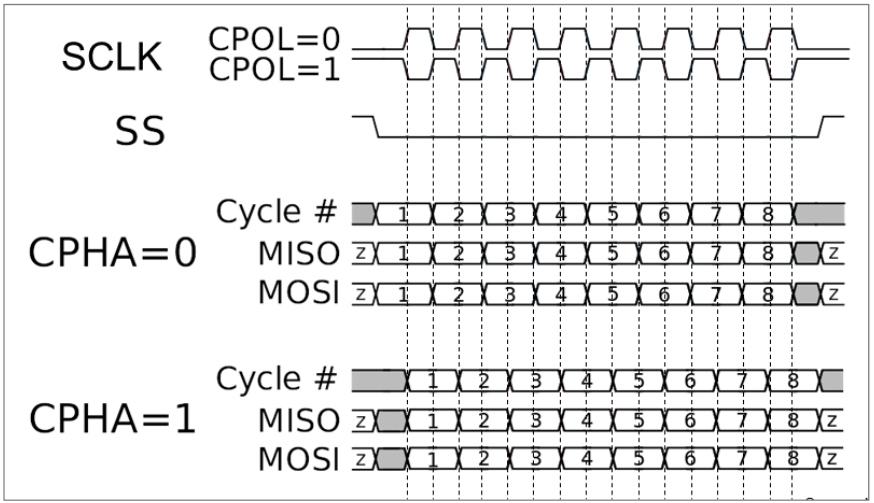
\includegraphics[width=\linewidth]{SPI_communication.png}

\begin{KR}{Analyzing SPI Communication}
\paragraph{Identify SPI mode}
\begin{itemize}
    \item Determine CPOL (Clock Polarity):
    \begin{itemize}
        \item CPOL=0: Clock idles low
        \item CPOL=1: Clock idles high
    \end{itemize}
    \item Determine CPHA (Clock Phase):
    \begin{itemize}
        \item CPHA=0: Data sampled on first edge (leading edge)
        \item CPHA=1: Data sampled on second edge (trailing edge)
    \end{itemize}
    \item Identify SPI mode from CPOL and CPHA:
    \begin{itemize}
        \item Mode 0: CPOL=0, CPHA=0
        \item Mode 1: CPOL=0, CPHA=1
        \item Mode 2: CPOL=1, CPHA=0
        \item Mode 3: CPOL=1, CPHA=1
    \end{itemize}
\end{itemize}

\paragraph{Draw timing diagram}
\begin{itemize}
    \item First, draw clock (SCLK) based on CPOL
    \item Draw chip select (SS\#) - active low
    \item Draw MOSI line with data from master to slave
    \item Draw MISO line with data from slave to master
    \item Indicate sampling edges based on CPHA:
    \begin{itemize}
        \item CPHA=0: Sample on rising edge if CPOL=0, falling edge if CPOL=1
        \item CPHA=1: Sample on falling edge if CPOL=0, rising edge if CPOL=1
    \end{itemize}
\end{itemize}

\paragraph{Calculate timing parameters}
\begin{itemize}
    \item Bit cell time = 1/clock\_frequency
    \item Frame time = (number\_of\_bits)/clock\_frequency
    \item Example: 8 bits at 100 kHz = 80 µs per frame
\end{itemize}
\end{KR}

\begin{example2}{SPI Timing Diagram Example}\\
Draw the timing diagram for an SPI transfer with:
\begin{itemize}
    \item Mode 3 (CPOL=1, CPHA=1)
    \item 8-bit data: MOSI = 0xA7, MISO = 0x37
    \item MSB first
    \item Clock frequency = 100 kHz
\end{itemize}
Mark all sampling edges on the diagram.

\tcblower
\paragraph{Solution:}
For Mode 3:
\begin{itemize}
    \item CPOL=1: Clock idles high
    \item CPHA=1: Data sampled on second edge (trailing edge)
    \item Sampling occurs on rising clock edges
\end{itemize}

Data values in binary:
\begin{itemize}
    \item MOSI: 0xA7 = 10100111
    \item MISO: 0x37 = 00110111
\end{itemize}

Bit cell time = 1/100 kHz = 10 µs

Timing diagram:
\begin{verbatim}
SS#   _|________________________________|_
          
SCLK  _|¯|_|¯|_|¯|_|¯|_|¯|_|¯|_|¯|_|¯|_|¯|_
          ^   ^   ^   ^   ^   ^   ^   ^
MOSI  ___|1|0|1|0|0|1|1|1|_________________
          
MISO  ___|0|0|1|1|0|1|1|1|_________________
\end{verbatim}

The arrows ($\wedge$) mark the sampling edges, which are the rising edges in Mode 3.

Total frame time = 8 bits × 10 µs = 80 µs.
\end{example2}

\subsection{I2C Communication}

\begin{concept}{I2C Timing} MSB first!\\
    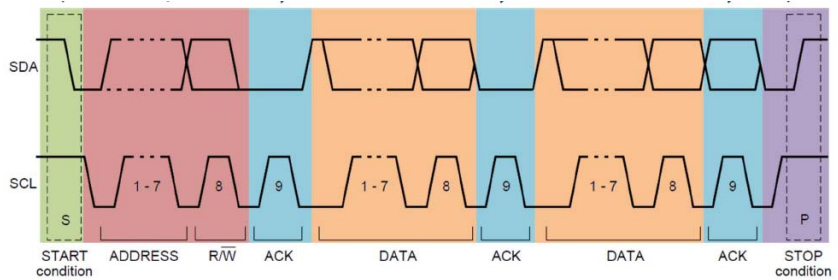
\includegraphics[width=\linewidth]{I2C_Timing.png}\\
    ACK = 0 $\rightarrow$ Übertragung erfolgreich\\
    ACK = 1 $\rightarrow$ Übertragung nicht erfolgreich
\end{concept}


\begin{KR}{Analyzing I2C Communication}
\paragraph{Identify I2C protocol elements}
\begin{itemize}
    \item Start condition: SDA falls while SCL is high
    \item Stop condition: SDA rises while SCL is high
    \item Data bit transfer: SDA stable while SCL is high
    \item Acknowledge (ACK): Receiver pulls SDA low during 9th clock cycle
    \item Not-acknowledge (NACK): SDA remains high during 9th clock cycle
\end{itemize}

\paragraph{Parse I2C frames}
\begin{itemize}
    \item First byte after start: 7-bit address + R/W bit
    \begin{itemize}
        \item R/W = 0: Write operation
        \item R/W = 1: Read operation
    \end{itemize}
    \item Check for ACK/NACK after each byte
    \item Data bytes follow (8 bits each)
    \item Master or slave can end transmission with STOP condition
\end{itemize}

\paragraph{Interpret timing diagram}
\begin{itemize}
    \item Examine SCL and SDA lines
    \item Identify start and stop conditions
    \item Group bits into bytes (8 bits + ACK/NACK)
    \item Determine if each byte is address or data
    \item Note the direction of data transfer
\end{itemize}
\end{KR}

\begin{example2}{I2C Communication Analysis}\\
Analyze the following I2C timing diagram and describe the transaction:

\begin{verbatim}
SCL  _____|¯¯¯|_|¯¯¯|_|¯¯¯|_|¯¯¯|_|¯¯¯|_|¯¯¯|_|¯¯¯|_|¯¯¯|_|¯¯¯|_|¯¯¯|...|¯¯¯|_|¯¯¯|_|¯¯¯|_|¯¯¯|_|¯¯¯|_|¯¯¯|_|¯¯¯|_|¯¯¯|_|¯¯¯|___
                     
SDA  ___\_|1|_|1|_|0|_|0|_|1|_|1|_|0|_|1|_|0|_\_|0|_|0|_|1|_|1|_|1|_|0|_|0|_|1|_/___
     Start                              ACK                 NACK  Stop
\end{verbatim}

\tcblower
\paragraph{Solution:}
The I2C transaction consists of:
\begin{enumerate}
    \item Start condition (SDA falls while SCL is high)
    \item First byte: 11001101 (data transmitted MSB first)
    \begin{itemize}
        \item This is the address byte: 1100110 (0x66) with R/W bit = 1 (read operation)
        \item Followed by an ACK (SDA pulled low during 9th clock cycle)
    \end{itemize}
    \item Second byte: 00111001 (data received from slave)
    \begin{itemize}
        \item This is data: 0x39 or 0x9C (depending on bit order interpretation)
        \item Followed by a NACK (SDA remains high during 9th clock cycle)
        \item NACK indicates that the master does not want to receive more data
    \end{itemize}
    \item Stop condition (SDA rises while SCL is high)
\end{enumerate}

The complete transaction is:
\begin{itemize}
    \item Master initiates communication with device at address 0x66
    \item Master requests to read from the device (R/W=1)
    \item Device acknowledges (ACK)
    \item Device sends one data byte (0x39 or 0x9C)
    \item Master signals end of transfer with NACK
    \item Master terminates communication
\end{itemize}
\end{example2}

\subsection{Protocol Comparison and Selection}

\begin{KR}{Selecting the Appropriate Serial Protocol}
\paragraph{Understand protocol characteristics}
\begin{itemize}
    \item \textbf{UART:}
    \begin{itemize}
        \item Point-to-point, full-duplex
        \item Asynchronous, no shared clock
        \item Simple wiring (2-3 wires)
        \item Moderate speed (up to ~5 Mbps)
    \end{itemize}
    \item \textbf{SPI:}
    \begin{itemize}
        \item Master-slave, full-duplex
        \item Synchronous with shared clock
        \item Multiple wires (MOSI, MISO, SCLK, SS)
        \item High speed (up to 50+ Mbps)
    \end{itemize}
    \item \textbf{I2C:}
    \begin{itemize}
        \item Multi-master, multi-slave
        \item Synchronous with shared clock
        \item Two wires (SCL, SDA)
        \item Medium speed (100 kbps, 400 kbps, up to 5 Mbps)
    \end{itemize}
\end{itemize}

\paragraph{Consider application requirements}
\begin{itemize}
    \item \textbf{Distance:}
    \begin{itemize}
        \item UART with RS-232 levels for longer distances
        \item SPI and I2C typically for on-board connections
    \end{itemize}
    \item \textbf{Speed:}
    \begin{itemize}
        \item SPI for highest speed requirements
        \item I2C for moderate speed with fewer pins
        \item UART for simpler, moderate speed connections
    \end{itemize}
    \item \textbf{Number of devices:}
    \begin{itemize}
        \item I2C for many devices on shared bus
        \item SPI for multiple devices but requires separate SS line for each
        \item UART typically for point-to-point (multiple UARTs needed for multiple devices)
    \end{itemize}
\end{itemize}

\paragraph{Evaluate protocol overhead}
\begin{itemize}
    \item \textbf{UART:}
    \begin{itemize}
        \item Start, stop, and optional parity bits
        \item Requires accurate clock timing
    \end{itemize}
    \item \textbf{SPI:}
    \begin{itemize}
        \item Minimal protocol overhead
        \item No addressing or acknowledgment
    \end{itemize}
    \item \textbf{I2C:}
    \begin{itemize}
        \item Start/stop conditions, addressing, and acknowledgment
        \item Higher protocol overhead but better error detection
    \end{itemize}
\end{itemize}

\paragraph{Consider hardware support}
\begin{itemize}
    \item Check if target microcontroller has hardware support for chosen protocol
    \item Consider available pins and alternate functions
    \item Evaluate available software libraries and drivers
    \item Consider power requirements (I2C has pull-up resistors that consume power)
\end{itemize}
\end{KR}

\begin{example2}{Serial Protocol Selection}\\
Select the most appropriate serial protocol for each of the following applications:
\begin{enumerate}
    \item A system needs to connect a microcontroller to three temperature sensors. The sensors are low-cost devices that should be replaceable without redesigning the PCB. Data rate requirement is low.
    \item A data acquisition system needs to transfer large amounts of data from an ADC to a microcontroller at 20 Mbps.
    \item A microcontroller needs to communicate with a PC via USB port.
    \item A control system needs to connect to four different devices at varying distances up to 30 meters in an electrically noisy industrial environment.
\end{enumerate}
\paragraph{Solution:}

1. \textbf{I2C is most appropriate for the temperature sensors:}
   \begin{itemize}
     \item Multiple devices (three sensors) can be connected to the same two wires
     \item Each sensor has a unique address, making them individually addressable
     \item Low data rate requirement is well within I2C capabilities
     \item Sensors can be replaced without changing connections (as long as addresses are configured properly)
     \item Reduced pin count (only SCL and SDA) simplifies PCB design
   \end{itemize}
   \vspace{2mm}
2. \textbf{SPI is most appropriate for the high-speed ADC:}
   \begin{itemize}
     \item 20 Mbps data rate exceeds practical I2C speeds and most UART configurations
     \item SPI can easily handle 20+ Mbps with direct hardware support
     \item SPI's full-duplex capability allows simultaneous control and data transfer
     \item Minimal protocol overhead maximizes throughput for large data amounts
     \item Hardware-based chip select ensures proper timing for ADC operations
   \end{itemize}
   \vspace{2mm}
3. \textbf{UART is most appropriate for PC communication:}
   \begin{itemize}
     \item UART is the typical protocol used with USB-to-serial converter chips
     \item Simple point-to-point connection is sufficient for PC communication
     \item Standard baudrates (9600, 115200, etc.) are well-supported by PC software
     \item No need for extra clock signals simplifies interfacing with USB adapters
     \item Asynchronous nature accommodates timing differences between systems
   \end{itemize}
   \vspace{2mm}
4. \textbf{RS-485 (based on UART) is most appropriate for the industrial control system:}
   \begin{itemize}
     \item RS-485 extends UART to longer distances (up to 1200m)
     \item Differential signaling provides excellent noise immunity in industrial environments
     \item Multi-drop capability allows connection to four devices on a single bus
     \item Higher voltage levels offer better signal integrity over 30m distances
     \item Various data rates possible depending on cable length (up to 10 Mbps at shorter distances)
     \item Industry standard protocol with wide hardware support
   \end{itemize}
\end{example2}